\chapter{Network Measurements}
\label{chp:measurements2}

This chapter will display the experiments conducted on data sending rate from the nRF52 to the Raspberry Pi in the form of and graphs, tables and figures to try to determine the most efficient combination of amount of data to send, sending frequency as well as protocols to use. 

%\section{temp/notes}

%Trying to understand the details of a capture in Wireshark. 

%Can fragmentation give us an advangate, if you can send more data pr header. 

%An empty char array sent over CoAP is 76 bytes. 
%19 bytes char array, 96 bytes
%21 bytes char array, 98 bytes. Adds only as much as needed. 
 



\section{Packet fragmentation}

In Internet Routing, \textit{fragmentation} is known as the action of splitting data into smaller packets, to satisfy the maximal limits of the different technologies or protocols used (e.g. \gls{ble} and \gls{6lowpan} in the network described in this thesis). Each of these packets needs header fields of a certain size, or other requirements.

To better understand fragmentation, imagine a train with carriages as shown in Figure \ref{fig:trainExample}. To be able to operate at all, the train needs a locomotive with an engine driver, a conductor and a cafe carriage. As soon as these things are already there, the company owning the train gets better and better off for every passenger buying a ticket. Lets assume that every carriage can carry 4 employees and 27 passengers, to make it directly comparable to the \gls{ble} packets in the network. Eventually all the carriages will be full, and a decision has to be made if it will be profitable to fit another carriage. It will in general be most profitable to use as many carriages as the locomotive can handle, and to fill up every carriage as much as possible. It will however not be a good idea to connect another carriage if there will only be one additional passenger sitting there, since the extra weight of the carriage adds unnecessary additional weight to the train set compared to the income. 

\begin{figure}[ht]
    \centering
    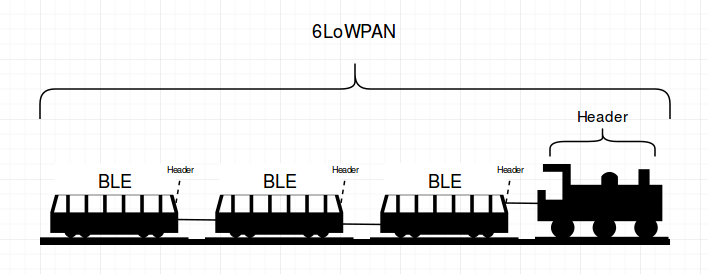
\includegraphics[scale=0.5]{trainExample.png}    
    \caption{Packet fragmentation - train comparison}
    \label{fig:trainExample}
\end{figure}

In this example, the locomotive and employees are the \gls{6lowpan} packet, that are needed no matter what to get the train working. Each additional carriage is a \gls{ble} packet. The goal is therefore to find the maximal number of passengers compared to the cost of adding additional carriages, in other words the maximal number of bytes compared to the number of packets sent. This is known as \textit{fragmentation}, to maximize \textit{goodput} vs \textit{throughput}. 

\subsection{Description of measurements}

The following sections will show experiments performed to to test if \textit{fragmentation} is a huge issiue when sending data through low energy networks, and which of the protocols described in chapter \ref{chp:background}  is the most efficient to use when the goal is to get as high \textit{googput} as possible. This will be done by sending data of constant length, capture packets using \textit{Wireshark}, and then increasing the packet size to see the changes. 

Before these experiements started, the expected results was that sending a small amount of data at a time would not be preferable, because of the needed bytes to set up the connection, header files and so on. It was not known how big the packages needed to be before it would be considered \textit{profitable} to send. 

When sending \gls{ble} packets over the network, observations from the system shows that the maximum packet size over \gls{ble} is 31 bytes. Each of these packages needs a header field of 4 bytes, meaning 27 bytes left for useful data. However, to start the connection at all, 76 byte is needed, meaning three \gls{ble} packets. The ratio between \textit{useful} and \textit{needed} (known as \textit{goodput} and \textit{throughput}) data transferred therefore start out very poorly if the payload sent is very small.

The best possible percentage of useful data we can hope to acheive will also be limited by this, 27 bytes goodput and 4 bytes header field, shown in the following calculation.  

\begin{align}
    27/31*100\% \approx 87,1 \%
\end{align}





In the actual system the number will quite certain be a lot lower than this. Both because header files in \gls{6lowpan} packages needs some bytes, and because of other limitations. 


\section{CoAP CON}

As explained in Chapter \ref{chp:architecture}, \gls{coap} CON messages can be sent quite frequently, but every message needs to get an \gls{ack} before the next message can be sent. This means that it is quite fast, but a lot of packets needs to be transported through to get usable data at the other end. 


\begin{figure}[ht]
    \centering
    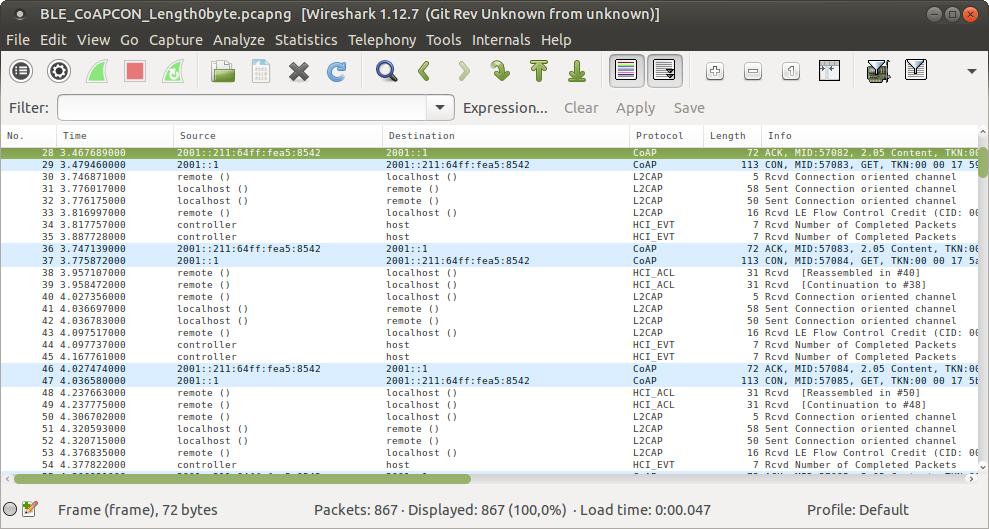
\includegraphics[width=\textwidth]{wiresharkCoAPCON0byte.png}    
    \caption{Wireshark capture, CoAP CON, 0 bytes goodput}
    \label{fig:coapCON0Wireshark}
\end{figure}

% Comment: Lage "utdrag", eller bare en liten del av Wireshark screenshot her, og legge hele i Appendix for å få det til å bli tydeligere? 


%something wrong
Figure \ref{fig:coapCON0Wireshark} shows an excerpt of a capture of packets in Wireshark. The full capture can be seen in the Appendix \ref{chp:appendix}. In this case an empty char array was sent, meaning an goodput equal to 0 byte. All of these bytes are therefore sent to route packages through the network. The maximum of 31 bytes per \gls{ble} packet have been exceeded twice, meaning that three packets needed to be sent. The first packet is labeled \textit{[Reassembled in \#40]}, the second \textit{[Continuation to \#38]} and the last \textit{Connection oriented channel}. After this, the \gls{ack} packages follows, two packages of 58 and 50 bytes, respectively. The last bytes received tells how many packages was completed, as a built in feature in \gls{ble}  \gls{hci}  and \gls{acl}. All of these packages can fit into one \gls{6lowpan} packet, since the total number of bytes are less than 270 bytes. 


\begin{figure}[ht]
    \centering
    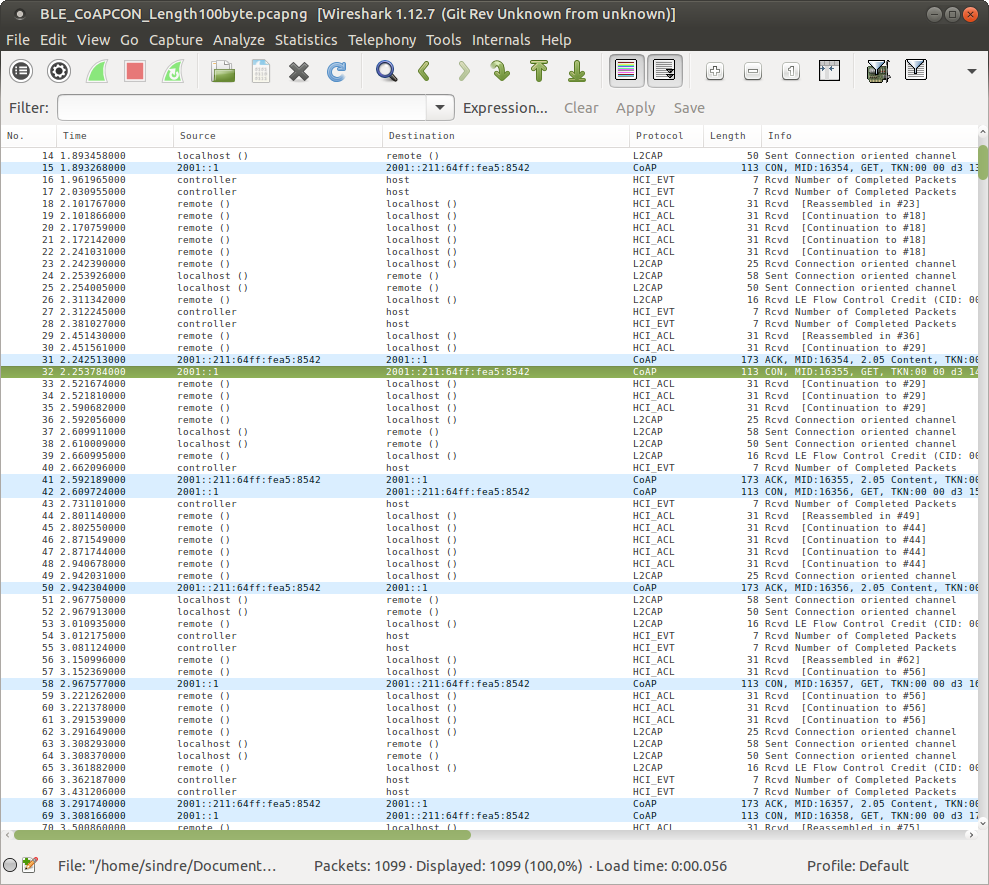
\includegraphics[width=\textwidth]{wiresharkCON100bytes.png}    
    \caption{Wireshark capture, CoAP CON, 100 bytes goodput}
    \label{fig:coapCON100Wireshark}
\end{figure}

In figure \ref{fig:coapCON100Wireshark}, 100 bytes of goodput is being sent through. The same basic packages needed are still there, but in addition the 100 bytes of data is added. This means adding more \gls{ble} packets, but also that the percentage of useful data sent through is a lot higher, approximatley 55 \% in this case. By doing several experiments like this, it was possible to create the graph in Figure \ref{fig:coapCON0200}. This shows the correlation between goodput and throughput compared to the number of packets sent, measured every 10th byte from 0 byte to 200 bytes large packets.


\begin{figure}[ht]
    \centering
    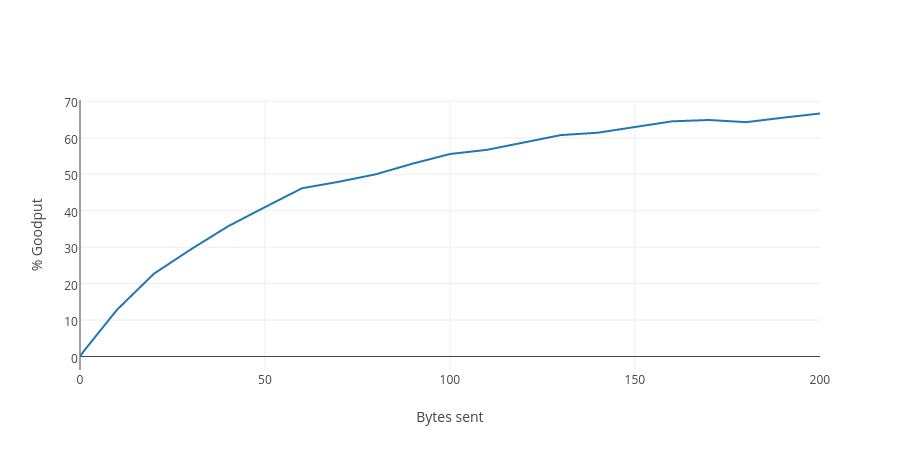
\includegraphics[scale=0.43]{CoAP_CONgraph2.png}    
    \caption{CoAP CON, 0-200 bytes sent}
    \label{fig:coapCON0200}
\end{figure}



In this particular case it makes no sense to send less than 50 bytes of useful data at once, since more than 50 \% of the bytes sent will be header files. This is comparable to having a locomotive and full crew at disposal, but only a few or none paying passengers. The best possible result is to have every carriage full, with 27 passengers and 4 employees. Since at least 4 bytes out of every 31 sent needs to be used to header information, the best possible result will be 87,1 \%, as shown in equation 4.1. Mathematically, this is described as a \textit{horizontal asymptote} since the distance between the graph and \textit{y = 87,1} will approach zero after an infinite number of bytes has been transferred. The graph will therefore converge to 87,1 \%, just as shown in figure \ref{fig:coapCON0200}, even before packet size of 200 bytes.  

\subsection{Discussion}

Even though this first test was done with a very limited amount of data transferred, it is easy to see that the curve clearly flattens out to the asymptote of the graph at 87,1 \%. The next step would normally be to transfer a larger amount of data, just to verify that these assumptions are true. The limitations of transfer rate is not nearly yet met by either \gls{ble} or \gls{6lowpan}. This test will therefore be explained in the next section. 


However, given that there is already a clear limit in figure \ref{fig:goodputThroughputGraph} even before the transfer rate reached 200 bytes, way before expected, it also makes sense to test various other transfer protocols. If it is possible to find a way of transportation that could give a higher mathematical maximum, and also get to this limit faster, it would be very profitable to the transfer of goodput in the system. Because the stable transfer interval at the moment is once every second, it also makes sense to test \gls{coap} with \gls{ack} for every packet, \textit{CON} instead of \textit{NON}. Maybe this means that the header files can be smaller for each packet, and that the useful amount of data sent true therefore will be higher. 


\subsection{CoAP CON with more data}

To see what happened when the limit of a \gls{6lowpan} packet was breached, tests was being set up to send bigger amounts of data than 200 bytes. This would also be a good way to prove that the percentage of goodput will converge to 87,1 \%, only considering \gls{ble} packets. The following test and examples will therefore send a fixed number of bytes at once from 0 to 1000 bytes (1 kB), with a 50 byte interval. As before, the messages are being sent as soon as possible, meaning approximately  four messages per second using \gls{coap} \gls{con}. 

\begin{figure}[ht]
    \centering
    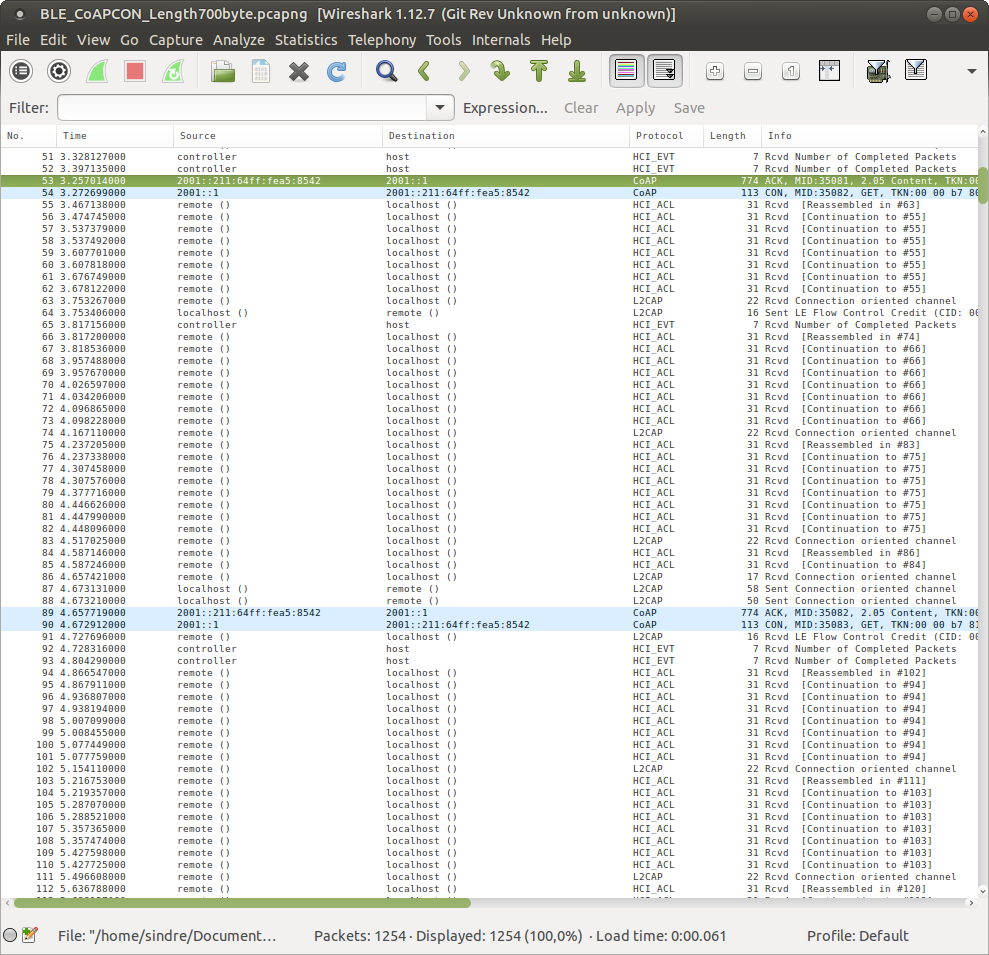
\includegraphics[width=\textwidth]{Wireshark700bytes2.png}    
    \caption{Wireshark capture, CoAP CON, 700 bytes goodput}
    \label{fig:coapCON700Wireshark}
\end{figure}

Figure \ref{fig:coapCON700Wireshark} shows one of these cases, where 700 bytes of data are being sent at once. In total 889 bytes are being sent, with a \gls{con} packet size of 774 bytes. This gives a percentage of goodput at 78.74 \%. The maximum packet length of a \gls{6lowpan} packet in this system of 270 bytes is therefore exceeded, as we can see in the figure. After 8 \gls{ble} packages of 31 bytes each has been sent, there is only room for 22 bytes in the last packet before the \gls{6lowpan} packet is full. This is repeated several times, once for each \gls{6lowpan} packet, until the last \gls{ble} packets at the size of 17 bytes. After this the standard packages for \gls{ack} and \textit{Number of completed packages} follows. This is in general a good example on how fragmentation of packets works in this system. 


\begin{figure}[ht]
    \centering
    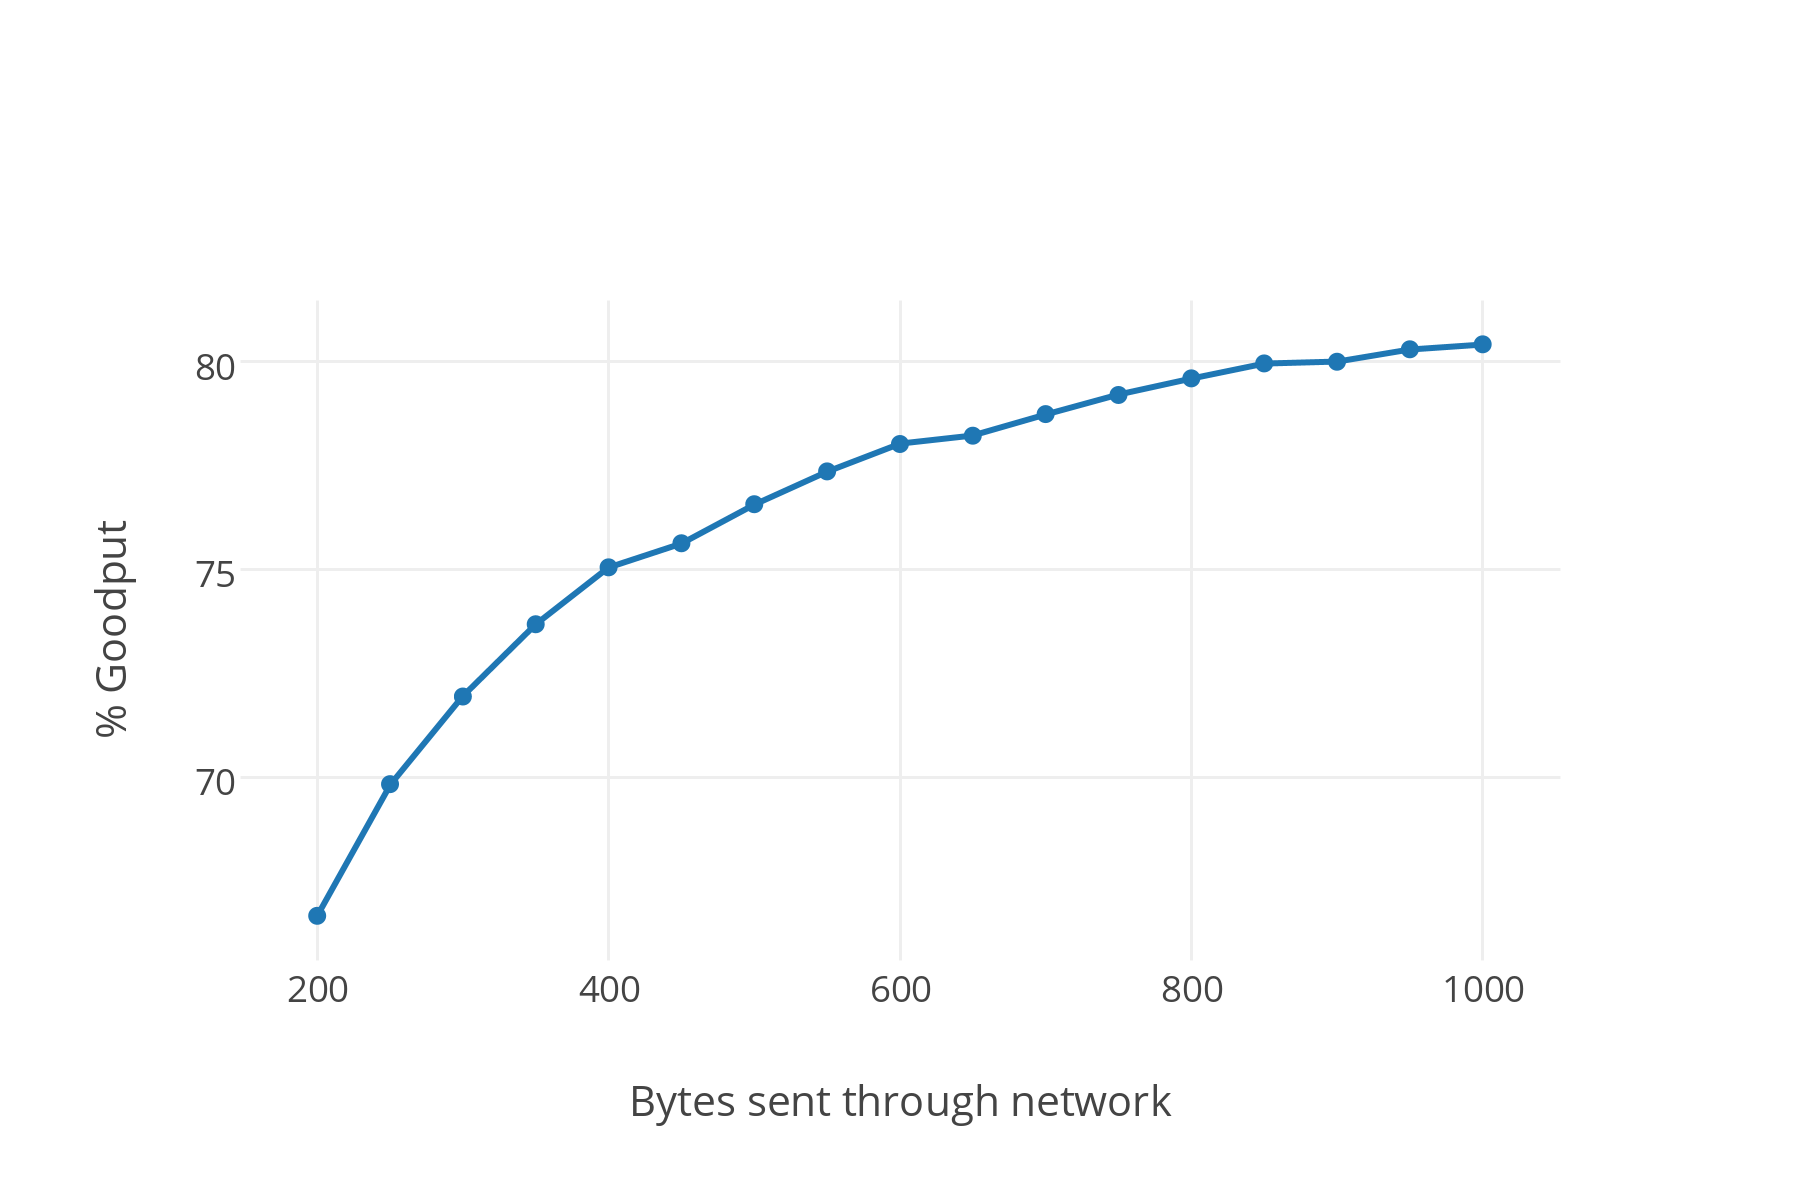
\includegraphics[width=\textwidth]{wireshark200-K_7.png}    
    \caption{CoAP CON plot, 200 bytes to 1 kB}
    \label{fig:plotCoAPCON200toK}
\end{figure}

Using these results it was possible to plot the graph in figure \ref{fig:plotCoAPCON200toK}. Here it is easy to see the same trends as in  \ref{fig:coapCON0200}, but in more detail over a wider span of bytes sent. These results are as expected after the previous tests, and in compliance with the calculations done in equation 4.1. 

In this example points in the graph was denoted every 50th byte sent. This gives us 


\section{CoAP NON}

In order to optimize the network, it makes sense to look into \gls{coap} \gls{non} in addition to \gls{con}. A \gls{non} request does not require a response in form of an \gls{ack}. This means that the 108 bytes sent to and handled by the end node can be skipped, which means less computational power and network capacity needed. This solution makes sense to use in networks where the demand for all data is low, since packets can be lost without the use of \glspl{ack}. 

The basic idea was here to check if data could be sent even faster without \glspl{ack}. However, this system turned out to be quite unstable at these high rates, and chased after running for a few seconds. To get the system stable the sending rate was slowed down to once every second. 

*Bilde 4 LEDs?*


\begin{figure}[ht]
    \centering
    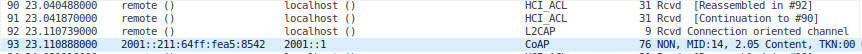
\includegraphics[scale=0.40]{coapNON0Bytes_PartOfWireshark.png}    
    \caption{CoAP NON 0 bytes Wireshark capture}
    \label{fig:NON0bytesPartOfWireshark}
\end{figure}

\subsection{CoAP NON, with more data}

A basic example of this connection is shown in figure \ref{fig:NON0bytesPartOfWireshark}. The entire Wireshark capture can be seen in Appendix \ref{chp:appendix}. This is directly comparable to figure \ref{fig:coapCON100Wireshark}, that shows a Wireshark capture of \gls{coap} \gls{con} packages. It is easy to see that a lot fewer packages needs to be sent using \gls{ble}, and no use of \glspl{ack}. The total amount of bytes sent is 31+31+9=71 bytes, meaning three \gls{ble} packages and one \gls{6lowpan} packet. This is less than half of what was needed using \gls{coap} \gls{con}, where the 108 \gls{ack} packages was needed in addition. The packets are still recognizable the same way as before, the first packet is labeled \textit{[Reassembled in \#40]}, the second \textit{[Continuation to \#38]} and the last \textit{Connection oriented channel}.

Fewer packages sent means less energy used, less network capacity needed and less computational power in the end node. Hopefully this will lead to a higher percentage of goodput compared to throughput as well. 


\begin{figure}[ht]
    \centering
    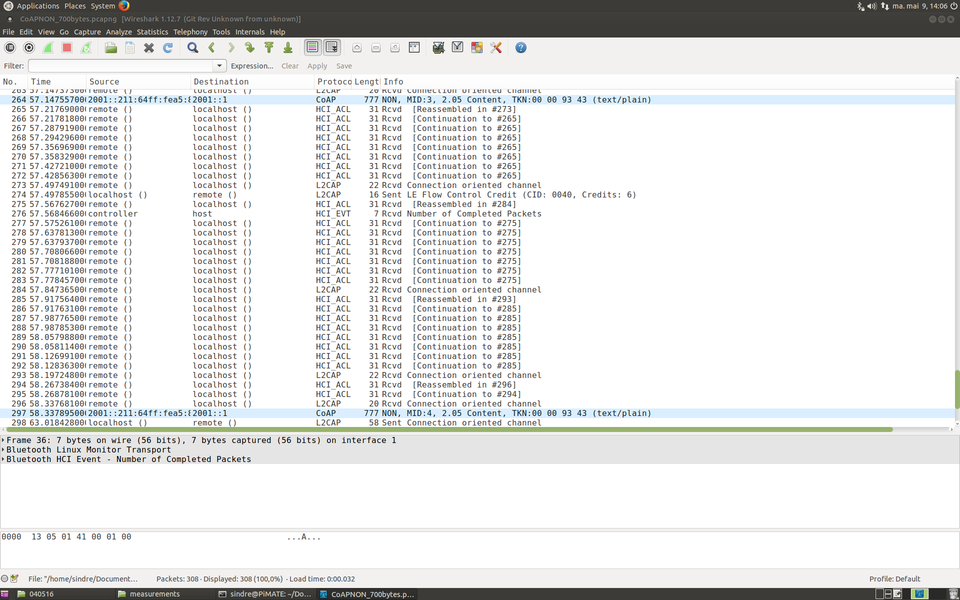
\includegraphics[scale=0.40]{rsz_1coapnon_wireshark700fullscreen.png}    
    \caption{CoAP NON 700 bytes Wireshark capture}
    \label{fig:NON7000bytesFullWireshark}
\end{figure}

The same in the form of a table: 

\begin{table}[]
\centering
\caption{Wireshark CoAP NON 700 bytes}
\label{coapNON700table}
\begin{tabular}{lllll}
\hline
Number & Time    & Protocol & Length & Info                             \\ \hline
264    & 57.1476 & CoAP     & 777    & NON, MID:3, 2.05 Content         \\
265    & 57.2177 & HCI\_ACL & 31     & Rcvd {[}Reassembled in \#273{]}  \\
266    & 57.2178 & HCI\_ACL & 31     & Rcvd {[}Continuation to \#265{]} \\
267    & 57.2879 & HCI\_ACL & 31     & Rcvd {[}Continuation to \#265{]} \\
268    & 57.2943 & HCI\_ACL & 31     & Rcvd {[}Continuation to \#265{]} \\
269    & 57.3570 & HCI\_ACL & 31     & Rcvd {[}Continuation to \#265{]} \\
270    & 57.3583 & HCI\_ACL & 31     & Rcvd {[}Continuation to \#265{]} \\
271    & 57.4272 & HCI\_ACL & 31     & Rcvd {[}Continuation to \#265{]} \\
272    & 57.4286 & HCI\_ACL & 31     & Rcvd {[}Continuation to \#265{]} \\
273    & 57.4975 & L2CAP    & 22     & Rcvd Connection oriented channel \\
274    & 57.4979 & L2CAP    & 16     & Sent LE Flow Control             \\
275    & 57.5676 & HCI\_ACL & 31     & Rcvd {[}Reassembled in \#284{]}  \\
276    & 57.5685 & HCI\_EVT & 7      & Rcvd Number of Completed Packets \\
277    & 57.5753 & HCI\_ACL & 31     & Rcvd {[}Continuation to \#275{]} \\
278    & 57.6378 & HCI\_ACL & 31     & Rcvd {[}Continuation to \#275{]} \\
279    & 57.6379 & HCI\_ACL & 31     & Rcvd {[}Continuation to \#275{]} \\
279    & 57.7080 & HCI\_ACL & 31     & Rcvd {[}Continuation to \#275{]} \\
280    & 57.7082 & HCI\_ACL & 31     & Rcvd {[}Continuation to \#275{]} \\
281    & 57.7771 & HCI\_ACL & 31     & Rcvd {[}Continuation to \#275{]} \\
282    & 57.7785 & HCI\_ACL & 31     & Rcvd {[}Continuation to \#275{]} \\
283    & 57.7785 & HCI\_ACL & 31     & Rcvd {[}Continuation to \#275{]} \\
284    & 57.8474 & L2CAP    & 22     & Rcvd Connection oriented channel \\
285    & 57.9176 & HCI\_ACL & 31     & Rcvd {[}Reassembled in \#293{]}  \\
286    & 57.9176 & HCI\_ACL & 31     & Rcvd {[}Continuation to \#285{]} \\
287    & 57.9878 & HCI\_ACL & 31     & Rcvd {[}Continuation to \#285{]} \\
288    & 57.9879 & HCI\_ACL & 31     & Rcvd {[}Continuation to \#285{]} \\
289    & 58.0580 & HCI\_ACL & 31     & Rcvd {[}Continuation to \#285{]} \\
290    & 58.0581 & HCI\_ACL & 31     & Rcvd {[}Continuation to \#285{]} \\
291    & 58.1270 & HCI\_ACL & 31     & Rcvd {[}Continuation to \#285{]} \\
292    & 58.1284 & HCI\_ACL & 31     & Rcvd {[}Continuation to \#285{]} \\
293    & 58.1972 & L2CAP    & 22     & Rcvd Connection oriented channel \\
294    & 58.2673 & HCI\_ACK & 31     & Rcvd {[}Reassembled in \#296{]}  \\
295    & 58.2688 & HCI\_ACL & 31     & Rcvd {[}Continuation to \#294{]} \\
296    & 58.3378 & L2CAP    & 20     & Rcvd Connection oriented channel \\
297    & 58.3379 & CoAP     & 777    & NON, MID:4, 2.05 Content         \\ \hline
\end{tabular}
\end{table}

Table \ref{coapNON700table} shows the packets captured in Wireshark when 700 bytes of data was sent through the network. 

%\begin{figure}[ht]
%    \centering
%    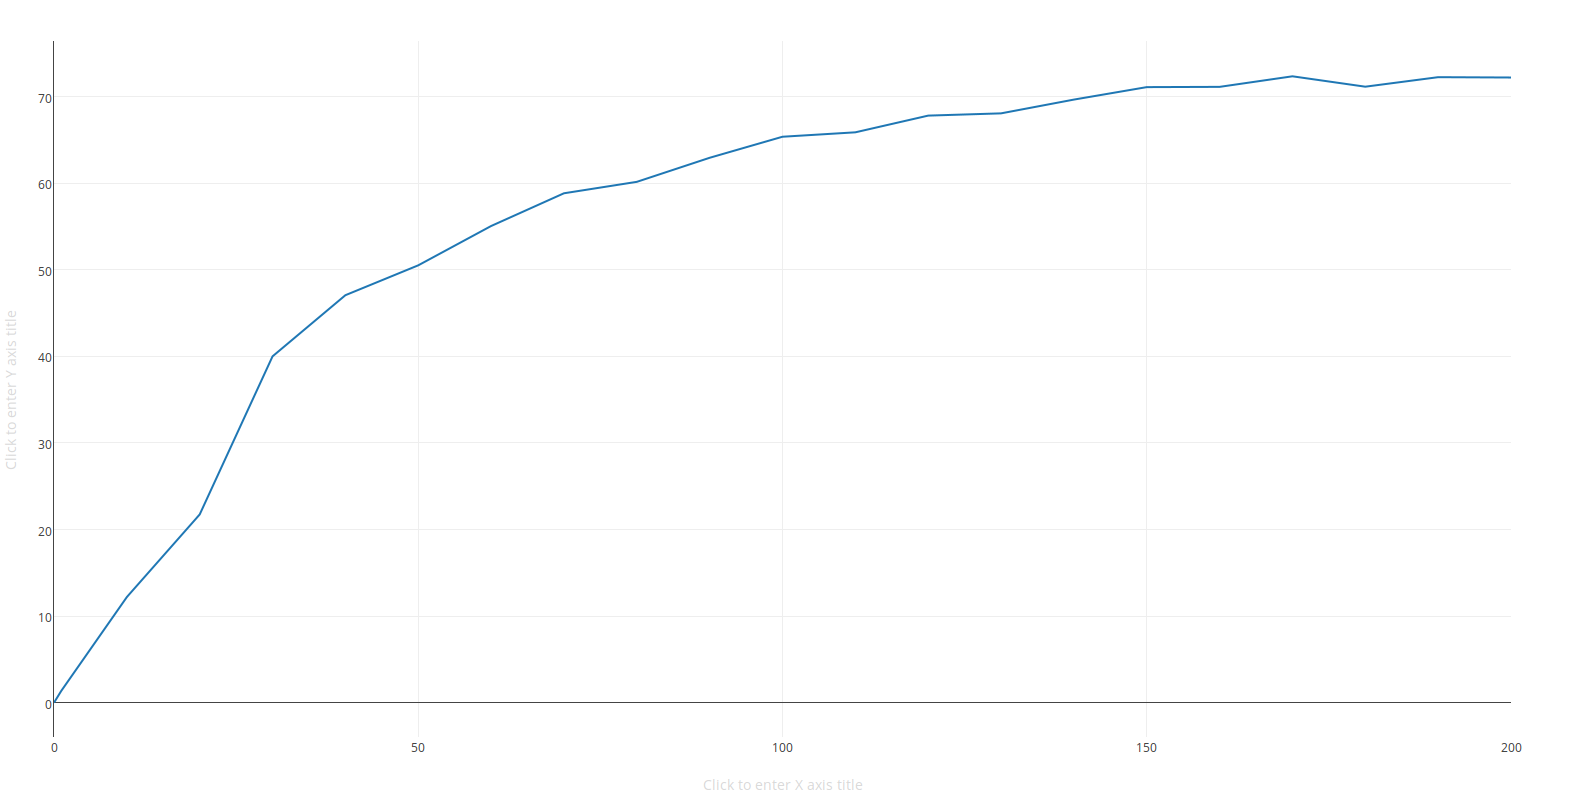
\includegraphics[scale=0.25]{graph1.png}    
%    \caption{Goodput compared to throughput in \%}
%    \label{fig:goodputThroughputGraph}
%\end{figure}



%\begin{figure}[ht]
%    \centering
%    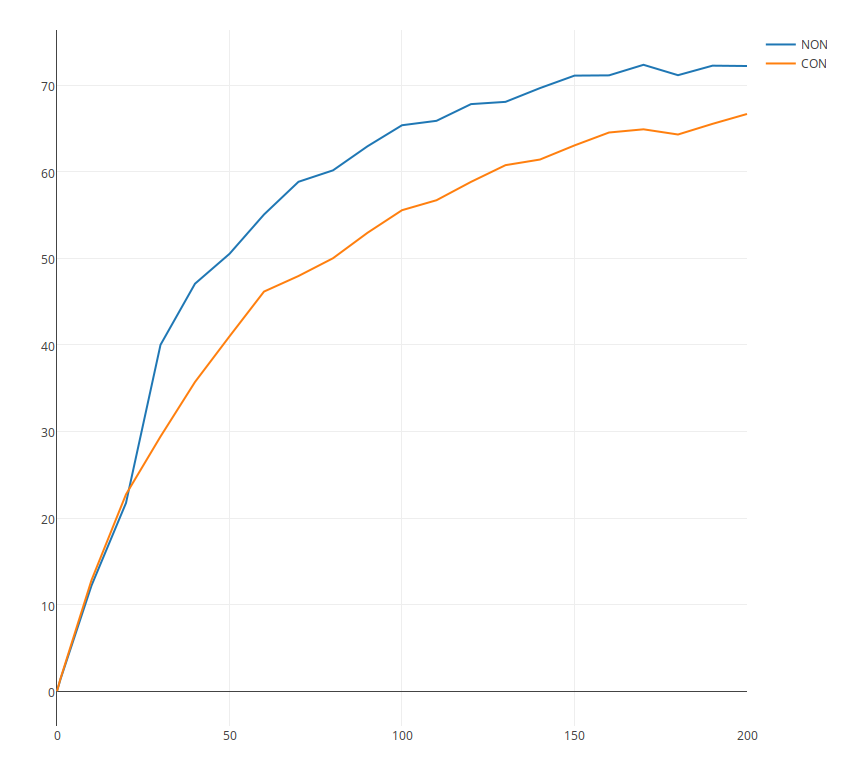
\includegraphics[scale=0.45]{CONvsNON1.png}    
%    \caption{CON vs NON}
%    \label{fig:CONvsNON}
%\end{figure}


\begin{figure}[ht]
    \centering
    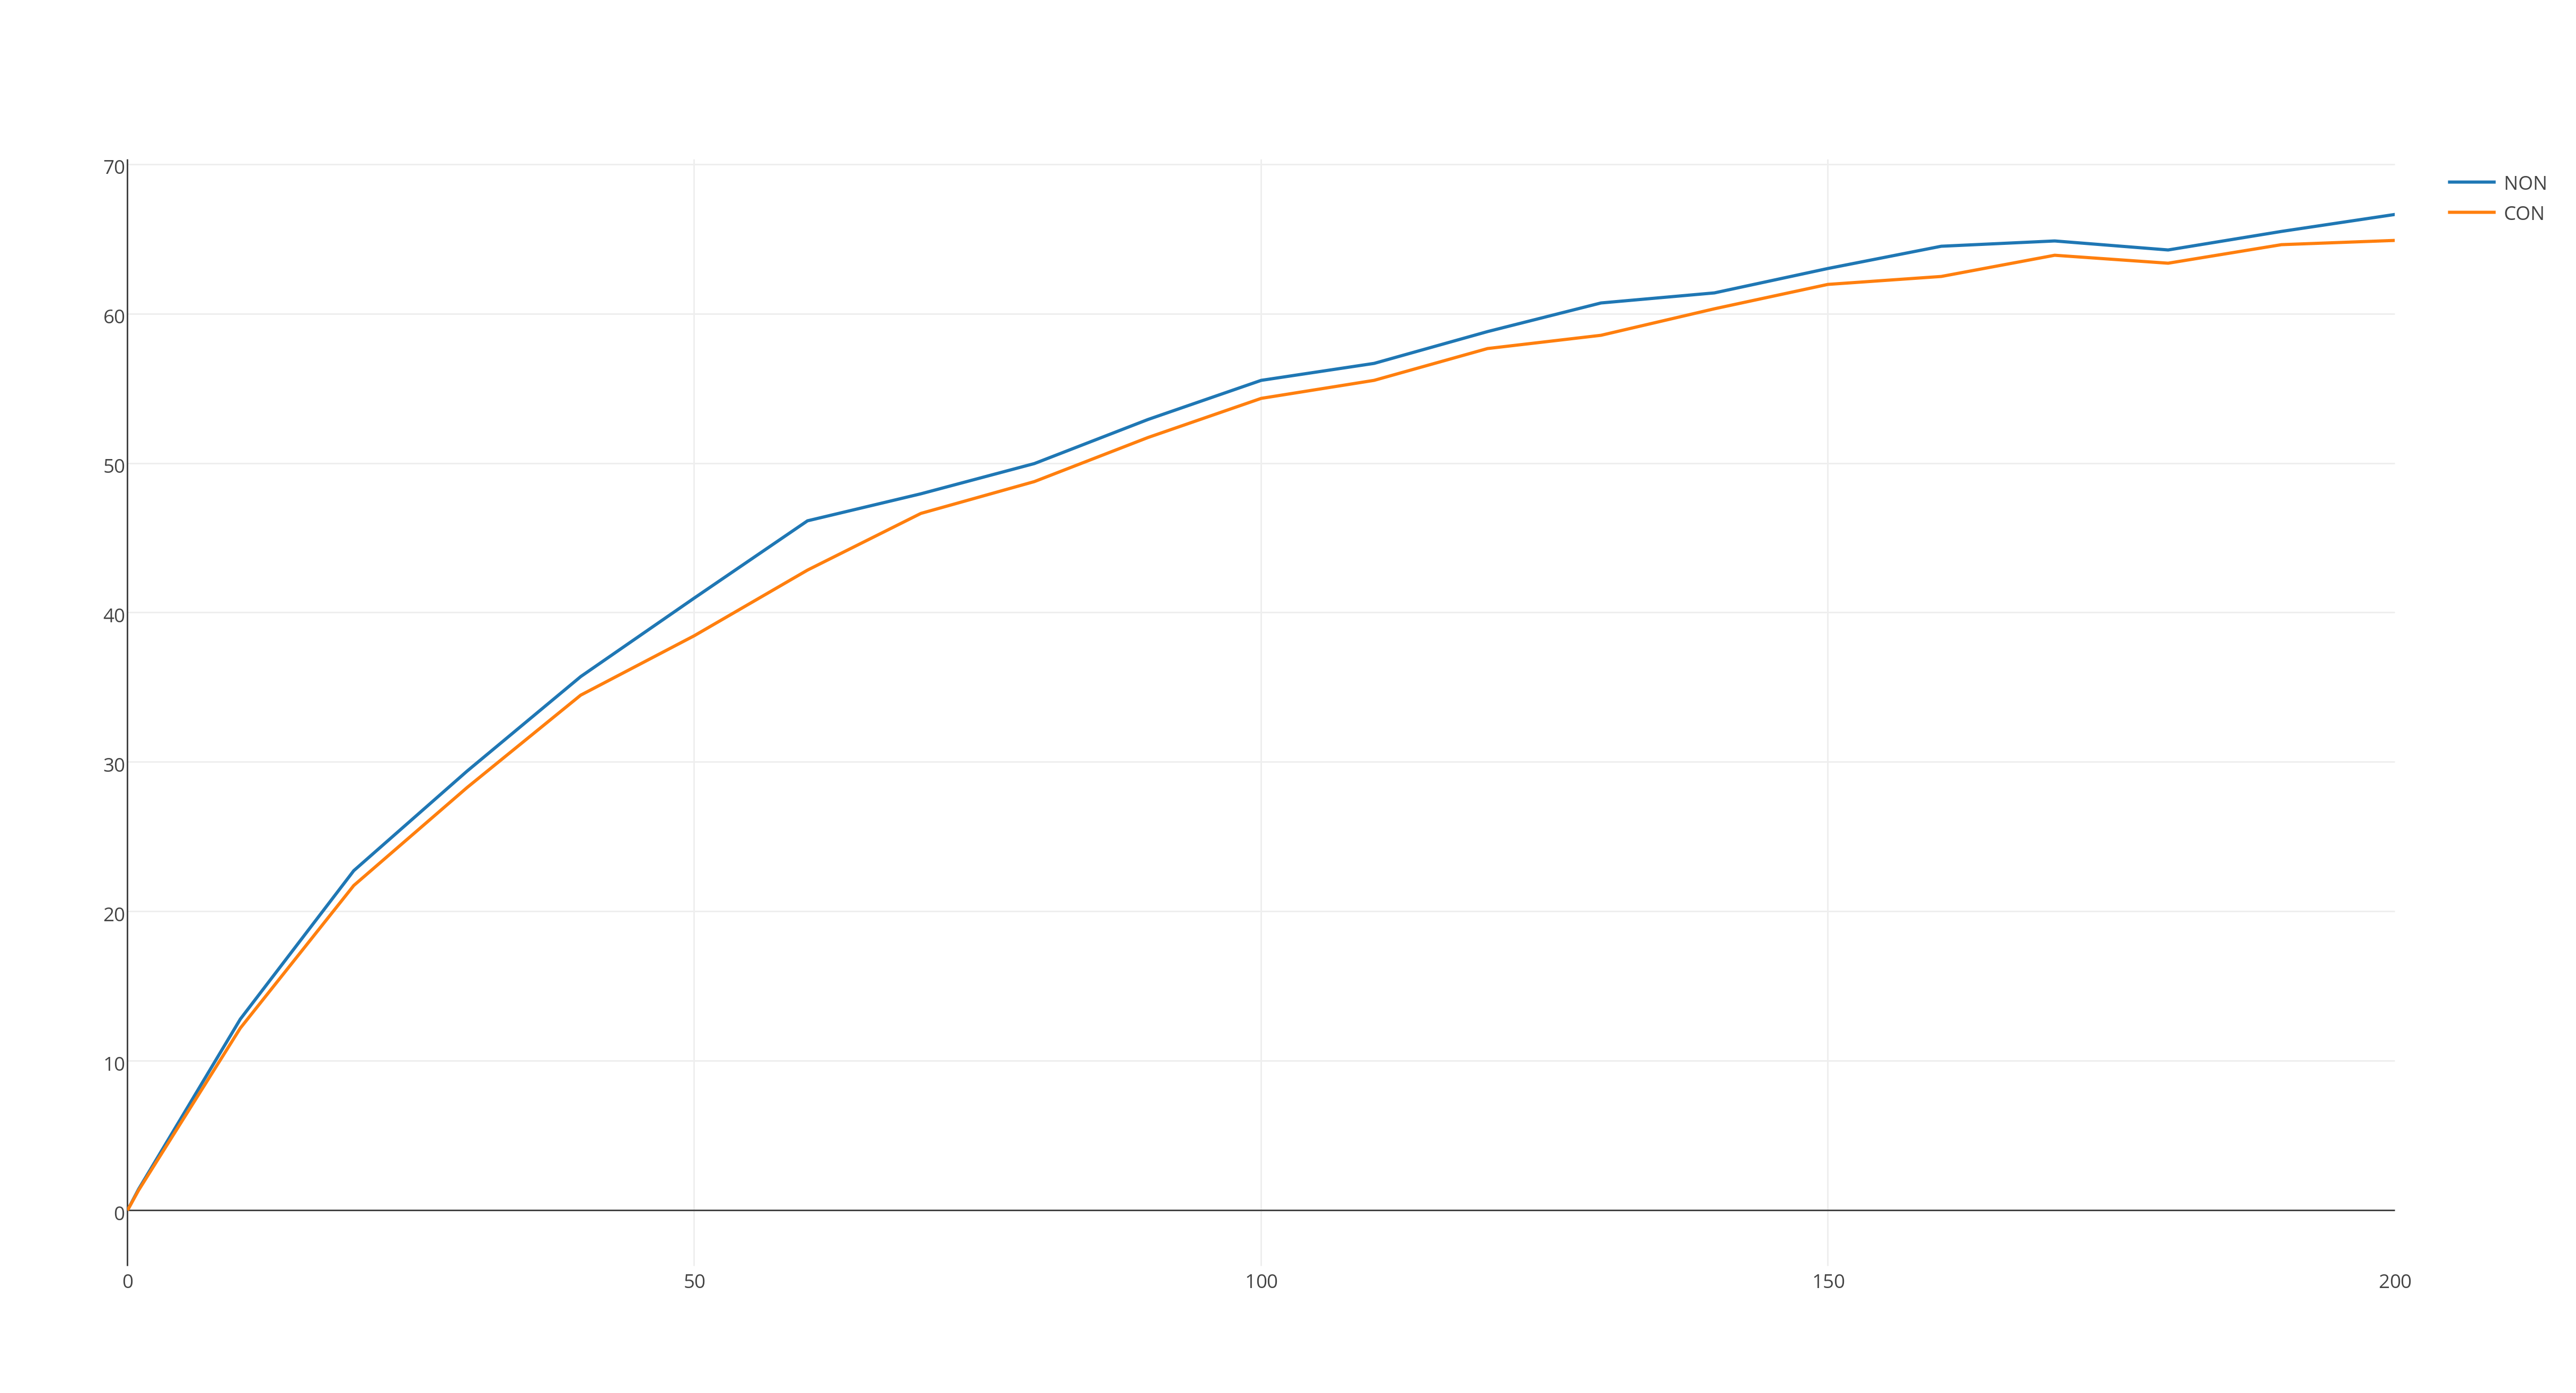
\includegraphics[scale=0.35]{NONvsCON_0-200.png}    
    \caption{CON vs NON 0-200 bytes}
    \label{fig:CONvsNON0-200}
\end{figure}


%\begin{figure}[ht]
%    \centering
%    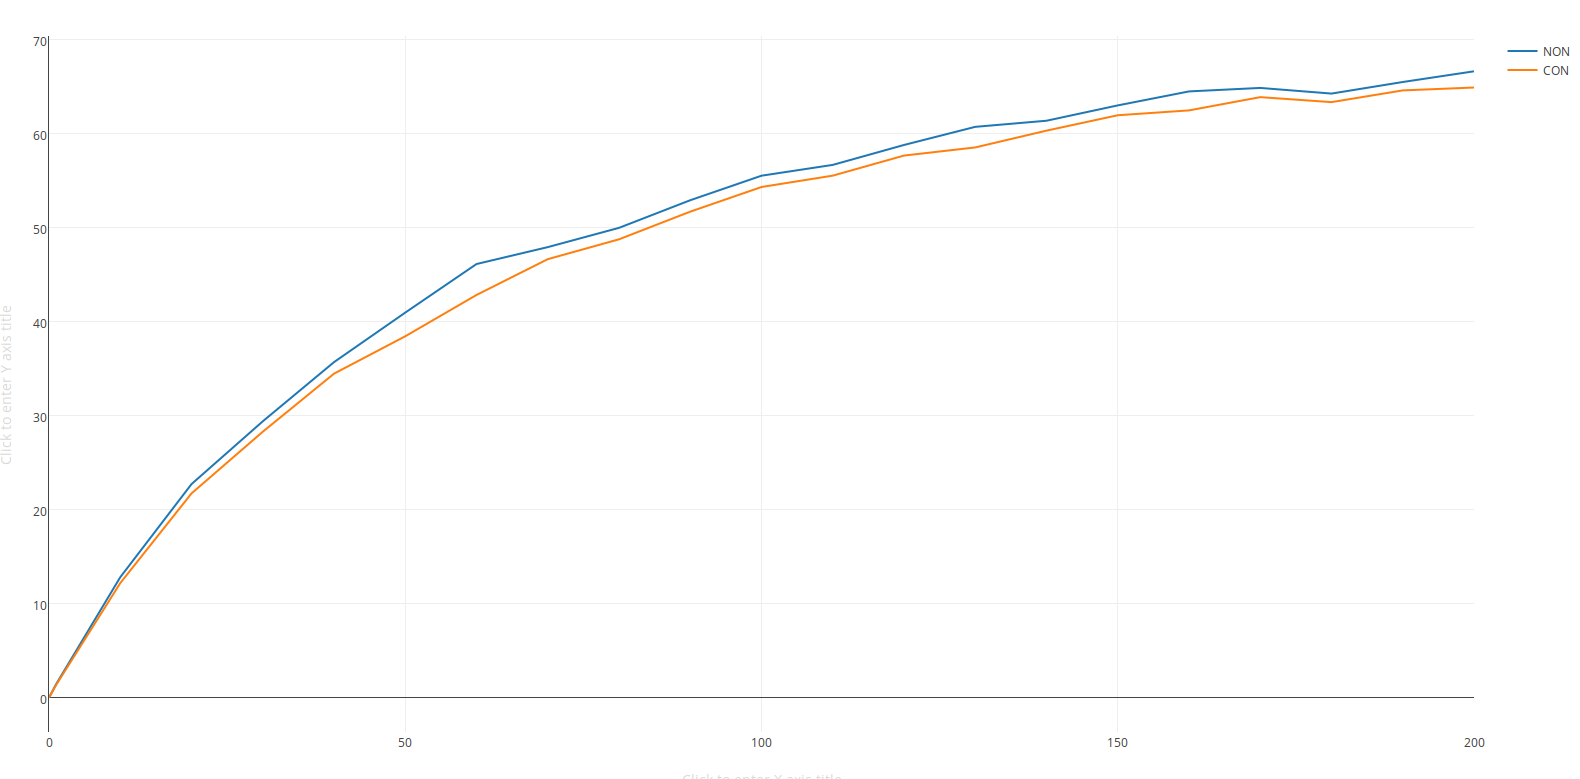
\includegraphics[scale=0.25]{CONvsNON0-200_2.png}    
%    \caption{CON vs NON 0-200 bytes number 2}
%    \label{fig:CONvsNON0-200}
%\end{figure}

\begin{figure}[ht]
    \centering
    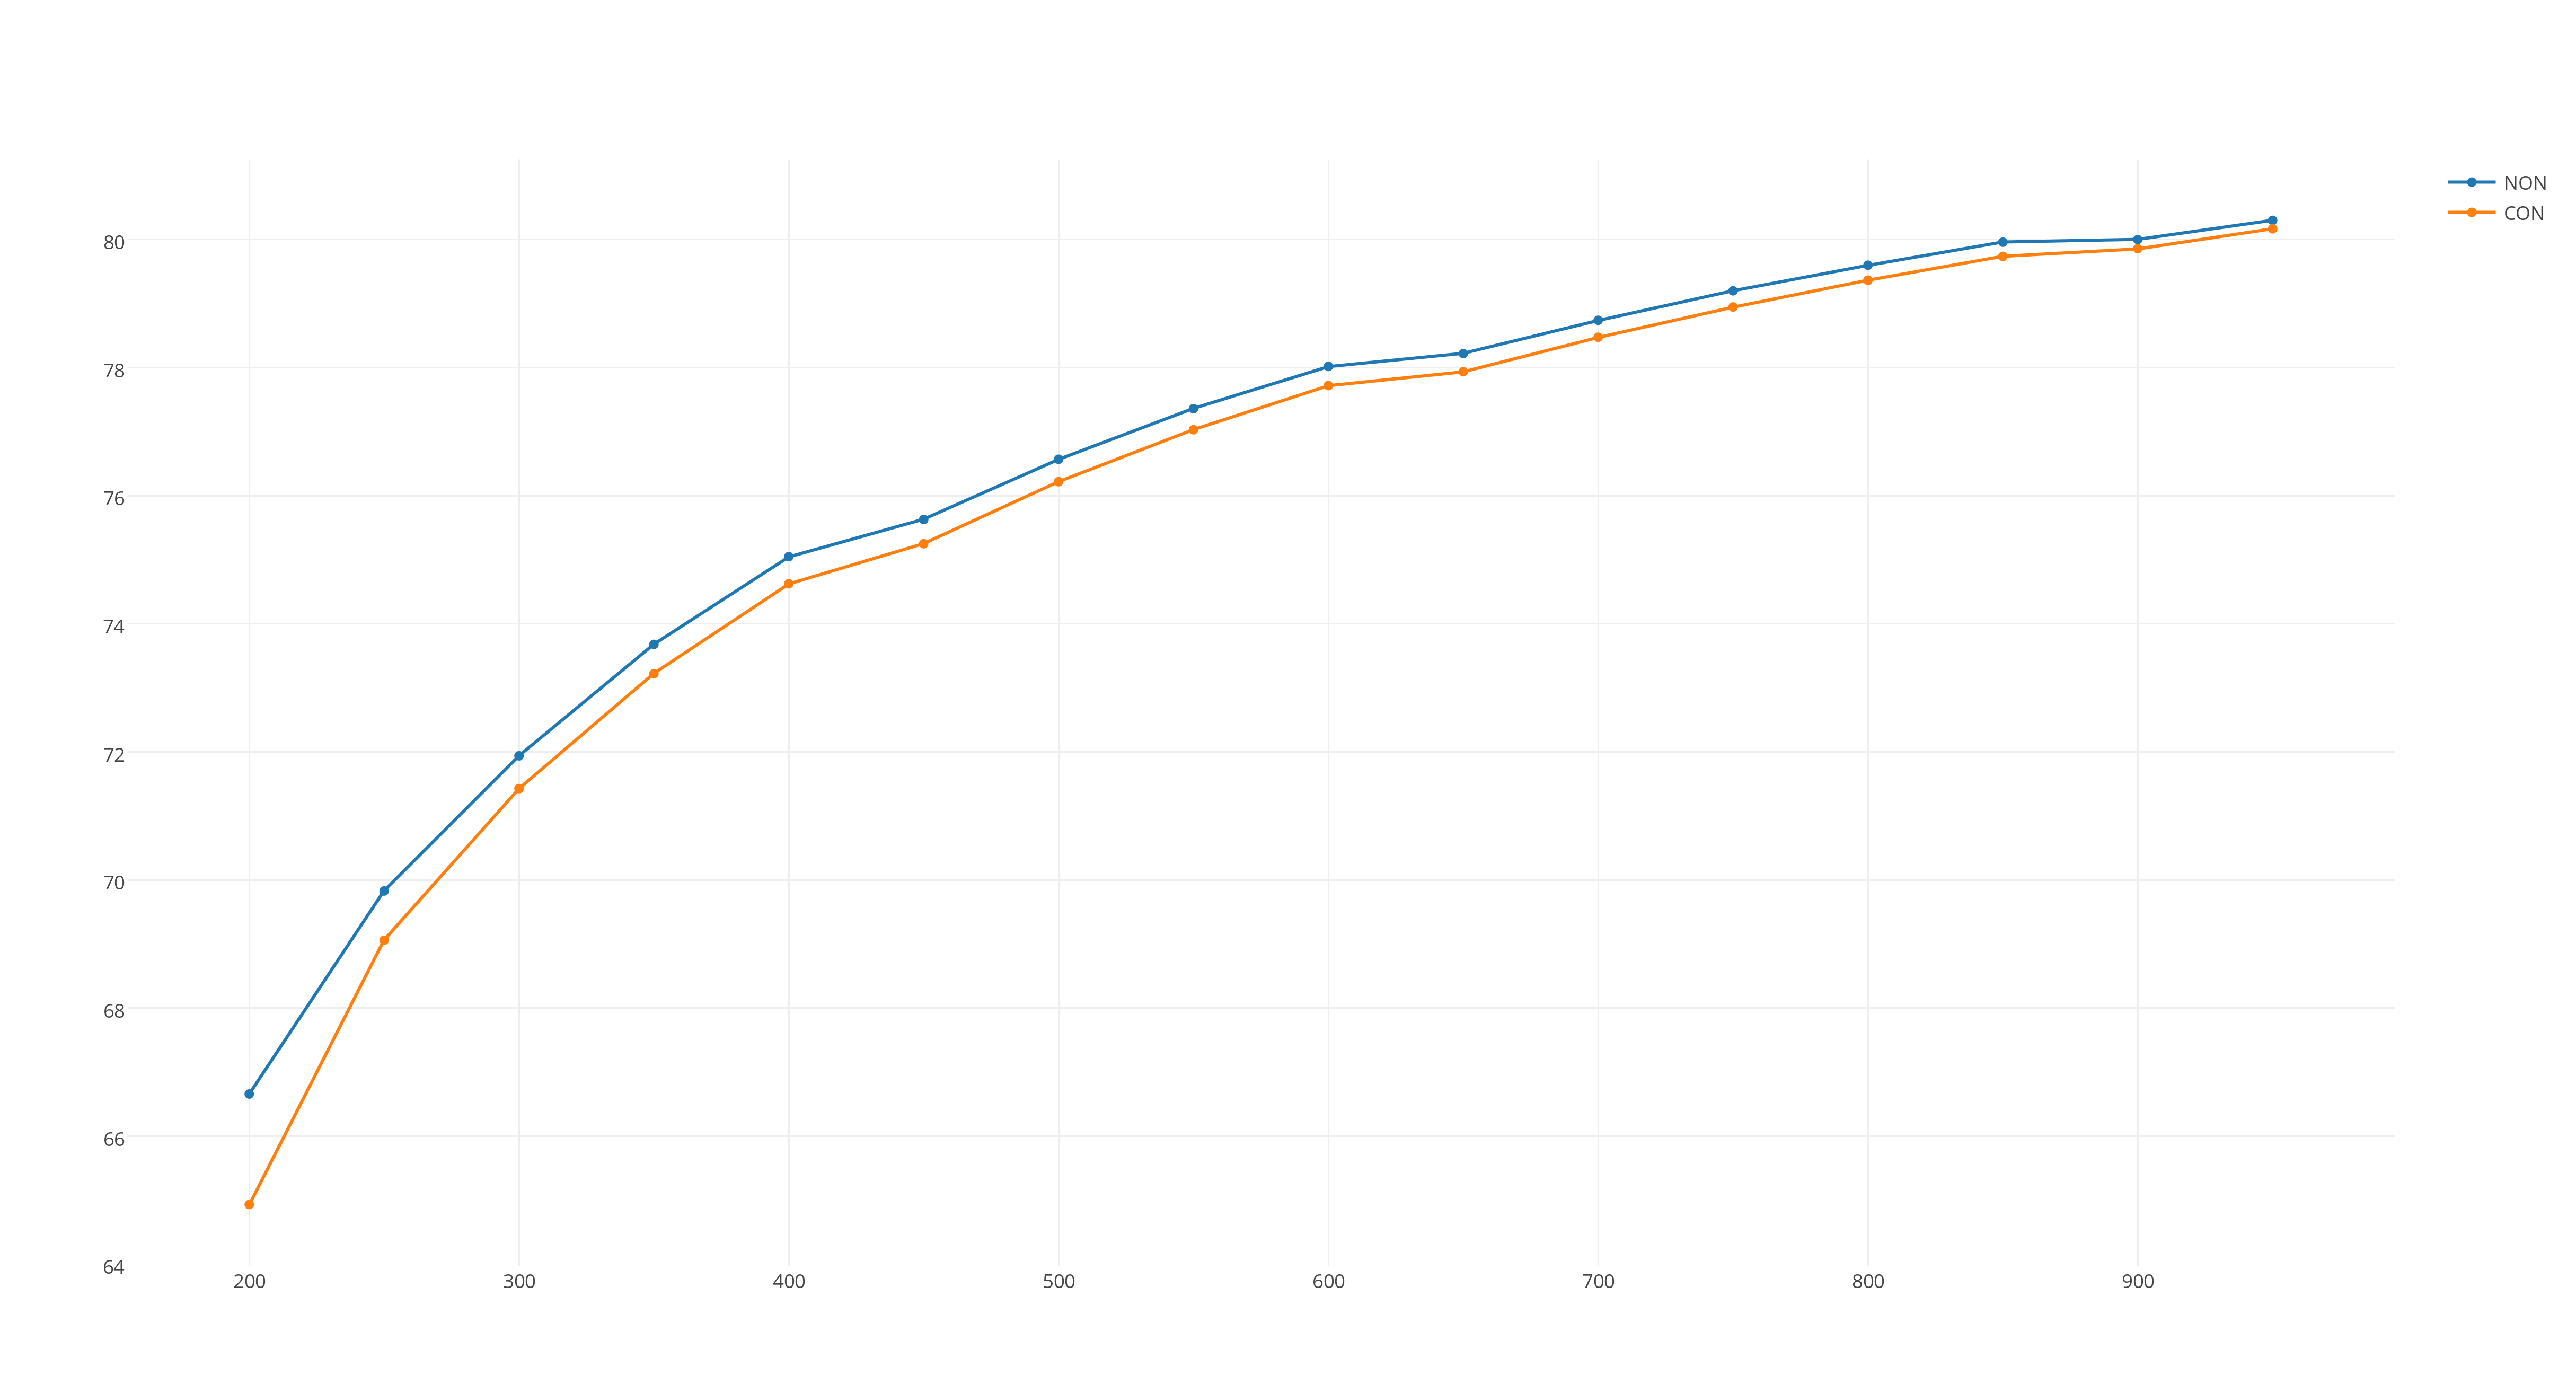
\includegraphics[scale=0.35]{NON-CON_200-950GRAPH.png}    
    \caption{CON vs NON 200-950 bytes}
    \label{fig:CONvsNON200-950}
\end{figure}


\subsection{Discussion}



\section{Time spent in network}

The previous tests shows 



\begin{align}
    27/31*100\% \approx 87,1 \%
\end{align}








